\documentclass[11pt]{article}

\usepackage{natbib,rotfloat,epsfig,setspace,amssymb,amsmath, comment}

\setlength{\hoffset}{0.2in}
\setlength{\voffset}{-0.6in}
\setlength{\textwidth}{6.0in}
\setlength{\evensidemargin}{0in}
\setlength{\oddsidemargin}{0in}
\setlength{\textheight}{8.5in}
\usepackage{graphicx}
\graphicspath{ {./images/} }

\begin{document}

\onehalfspace

\title{Economics 512 -- Empirical Methods \\ Homework 7}
\author{Due Wednesday, February 11, 2019}
\date{}
\maketitle

\section*{Learning By Doing Duopoly.}

The exercise below is inspired by the learning-by-doing model of Besanko,
Doraszelski, Kryukov, and Satterthwaite (2010, Econometrica).

Two ex-ante identical firms are characterized by their production ``know-how'' $\omega
\in \{1,\ldots,L\}$ which summarizes the firms accumulated technical knowledge. 
The marginal cost of production, $c(\omega)$,
depends on this stock of know-how. In particular, the monopolist
faces a learning curve given by
\begin{equation*}
c(\omega )=\left\{
\begin{array}{ccc}
\kappa \omega ^{\eta } & \mbox{ if } & 1\leq \omega <l, \\
\kappa l^{\eta } & \mbox{ if } & l\leq \omega \leq L,%
\end{array}
\right.
\end{equation*}
where $\eta =\frac{\ln \rho }{\ln 2}$ for a learning curve with a
slope of $\rho $ percent, $\kappa $ is the marginal cost with
minimal know-how (normalized to be $\omega =1$), and $l<L$
represents the stock of know-how at which the firm reaches the
bottom of its learning curve.

The model is cast in discrete time and has an infinite horizon to
avoid end effects. I first describe the product market and then turn
to pricing dynamics. Unlike the quality ladder model, the
learning-by-doing model cannot be broken down in a static and a
dynamic part.

There are two firms.  The state space is thus
$\Omega \in \{1,\ldots,L\}^2$. I refer to $\mathbf{\omega}=(\omega_1,\omega_2)$ 
as the state of the industry and to $\omega_n$ as the state of firm $n$.

\paragraph{Product market.}

Each periods, firms compete to make a sale.  The probability that firm $n$ makes the sale is
\begin{equation*}
D_{n}(p_{1},p_{2})=\frac{\exp \left( v-p_{n}\right) }{1+\sum_{k=1}^2\exp\left(
v-p_{k}\right)  },
\end{equation*}%
where $v$ is a quality of the good.

\paragraph{Pricing dynamics.}

Each firm's state $\omega $ represents its know-how in the
present period. Its know-how in the subsequent period,
$\omega^\prime$, depends on whether or not it makes a sale and on
whether or not its stock of know-how depreciates.

The probability that the stock of know-how depreciates is $\Pr(f=1)=\Delta
(\omega)=1-(1-\delta)^{\omega}$, where $\delta \in [0,1]$. This
specification is conceptually similar to the deterministic
\textquotedblleft capital-stock\textquotedblright\ models of
depreciation employed in the empirical work on organizational
forgetting, where the depreciation
of know-how increases as the firm's stock of know-how increases.

The law of motion for each firm's
stock of know-how is
$$
\omega^\prime=\omega+q-f,
$$
where $q\in\{0,1\}$ indicates whether the monopolist makes a sale and
$f\in\{0,1\}$ represents organizational forgetting.
The monopolist's
stock of know-how therefore changes according the transition function
\begin{equation*}
\Pr (\omega^{\prime }|\omega,q)=\left\{
\begin{array}{cll}
1-\Delta (\omega) & \mbox{ if } & \omega^{\prime
}=\omega+q, \\
\Delta (\omega) & \mbox{ if } & \omega^{\prime
}=\omega+q-1,%
\end{array}
\right.
\end{equation*}
At the upper and lower boundaries of the state space, I take the
transition function to be $\Pr (L|L,q=1)=1$ and $\Pr (1|1,q=0)=1$,
respectively.

The Bellman equation for firm $n$ is
\begin{equation*}
V_n(\mathbf{\omega})=\max_{p_n }
D_n(p_n,p_{-n}(\mathbf{\omega}))(p_n-c(\omega_n))+\beta\sum_{k=0}^2D_k(p_n,p_{-n}(\mathbf{\omega}))W_{nk}(\mathbf{\omega}),
\end{equation*}%
where $p_{-n}(\mathbf{\omega})$ is the
rival's pricing strategy, and
\begin{eqnarray*}
W_{n0}(\mathbf{\omega}) & = & \sum_{\omega_1^\prime=1}^L\sum_{\omega_2^\prime=1}^LV_n(\mathbf{\omega}^\prime)\Pr(\omega_1^\prime|\omega_1,q_1=0)\Pr(\omega_2^\prime|\omega_2,q_2=0), \\
W_{n1}(\omega) & = & \sum_{\omega_1^\prime=1}^L\sum_{\omega_2^\prime=1}^LV_n(\mathbf{\omega}^\prime)\Pr(\omega_1^\prime|\omega_1,q_1=1)\Pr(\omega_2^\prime|\omega_2,q_2=0), \\
W_{n2}(\omega) & = & \sum_{\omega_1^\prime=1}^L\sum_{\omega_2^\prime=1}^LV_n(\mathbf{\omega}^\prime)\Pr(\omega_1^\prime|\omega_1,q_1=0)\Pr(\omega_2^\prime|\omega_2,q_2=1)
\end{eqnarray*}
is the expectation of the value function of firm $n$ conditional on the buyer purchasing good $k\in\{0,1,2\}$ (good $0$ is the outside good).

The pricing strategy of firm $n$ is given by
\begin{equation*}
p_n\left( \omega \right)
=\arg\max_{p_n}D_n(p_n,p_{-n}(\mathbf{\omega}))(p_n-c(\omega_n))+\beta\sum_{k=0}^2D_k(p_n,p_{-n}(\mathbf{\omega}))
W_{nk}(\mathbf{\omega}).
\end{equation*}%
Let
$h_n(p_n)=D_n(p_n,p_{-n}(\mathbf{\omega}))(p_n-c(\omega_n))+\beta\sum_{k=0}^2D_k(p_n,p_{-n}(\mathbf{\omega}))W_{nk}(\mathbf{\omega})$
denote the maximand on the RHS of the Bellman equation.
$h_n(p_n)$ is strictly quasi-concave and the price choice $p_n(%
\mathbf{\omega})$ is therefore unique. It is found by numerically solving $\frac{\partial h_n}{\partial p_n}=0$ or, equivalently,
\begin{gather*}
0=1-(1-D_n(p_n,p_{-n}(\mathbf{\omega})))\left(p_n-c(\omega_n)\right)-\beta W_{nn}(\mathbf{\omega})\\
+ \beta\sum_{k=0}^2D_k(p_n,p_{-n}(\mathbf{\omega}))W_{nk}(\mathbf{\omega}).
\end{gather*}

\paragraph{Equilibrium.}

The primitives are symmetric. I therefore restrict attention to
symmetric Markov perfect equilibria (MPE). Such a MPE is
characterized by a value function $V(\omega)$ and a policy function
$p(\omega)$ such that, if $V(\omega)$ is firm 1's value function,
then firm 2's value function is given by
$V_{2}(\omega_1,\omega_2)=V(\omega_2,\omega_1)$. Similarly, if
$p(\omega)$ is firm 1's policy function, then firm 2's policy
function is given by
$p_{2}(\omega_1,\omega_2)=p(\omega_2,\omega_1)$. Existence of a
symmetric MPE in pure strategies follows from the arguments in
Doraszelski and Satterthwaite (2010) provided that prices are bounded.

\paragraph{Algorithm.}

To compute the MPE, Pakes and McGuire (1995) suggest an algorithm that
essentially adapts value function iteration to dynamic games. The
algorithm proceeds as follows:
\begin{enumerate}
\item Make initial guesses for the value and policy functions (or, more precisely, $L\times L$ matrices), $\mathbf{V}^0$
and $\mathbf{p}^0$, choose a stopping criterion $\epsilon>0$, and
initialize the iteration counter to $l=1$.

\item For all states $\mathbf{\omega} \in \Omega$ compute
\begin{equation*}
p^{l+1}\left( \mathbf{\omega} \right)
=\arg\max_{p_1}D_1(p_1,p_2^l(\omega_2,\omega_1))(p_1-c(\omega_1))+\beta\sum_{k=0}^2D_k(p_1,p_2^l(\omega_2,\omega_1))
W^l_{k}(\mathbf{\omega})).
\end{equation*}%
and
\begin{equation*}
V^{l+1}(\mathbf{\omega})=
D_1(p_1^{l+1}(\mathbf{\omega}),p_2^l(\omega_2,\omega_1))(p_1^{l+1}(\mathbf{\omega})-c(\omega_1))+\beta\sum_{k=0}^2
D_k(p_1^{l+1}(\mathbf{\omega}),p_2^l(\omega_2,\omega_1))W^l_{n}(\mathbf{\omega}).
\end{equation*}%
where
\begin{eqnarray*}
W^l_{0}(\mathbf{\omega}) & = & \sum_{\omega_1^\prime=1}^L\sum_{\omega_2^\prime=1}^LV^l(\mathbf{\omega}^\prime)\Pr(\omega_1^\prime|\omega_1,q_1=0)\Pr(\omega_2^\prime|\omega_2,q_2=0), \\
W^l_{1}(\mathbf{\omega}) & = & \sum_{\omega_1^\prime=1}^L\sum_{\omega_2^\prime=1}^LV^l(\mathbf{\omega}^\prime)\Pr(\omega_1^\prime|\omega_1,q_1=1)\Pr(\omega_2^\prime|\omega_2,q_2=0), \\
W^l_{2}(\mathbf{\omega}) & = & \sum_{\omega_1^\prime=1}^L\sum_{\omega_2^\prime=1}^LV^l(\mathbf{\omega}^\prime)\Pr(\omega_1^\prime|\omega_1,q_1=0)\Pr(\omega_2^\prime|\omega_2,q_2=1).
\end{eqnarray*}

\item If
\begin{displaymath}
\max_{\mathbf{\omega}\in\Omega}\left|
\frac{V^{l+1}(\mathbf{\omega})-V^l(\mathbf{\omega})}{1+|V^{l+1}(\mathbf{\omega})|} \right|
<\epsilon \quad \wedge \quad \max_{\mathbf{\omega}\in\Omega}\left|
\frac{p^{l+1}(\mathbf{\omega})-p^l(\mathbf{\omega})}{1+|p^{l+1}(\mathbf{\omega})|} \right|
<\epsilon
\end{displaymath}
then stop; else increment the iteration counter $l$ by one and go to
step 2.
\end{enumerate}

Unlike value function iteration for single-agent dynamic programming
problems, there is no guarantee that the above algorithm converges.
If it fails to converge, a trick that often works is to go through
an additional dampening step before returning to step 2. This
dampening step assigns
\begin{eqnarray*}
\mathbf{V}^{l+1} & \leftarrow & \lambda \mathbf{V}^{l+1} +(1-\lambda) \mathbf{V}^{l}, \\
\mathbf{p}^{l+1} & \leftarrow & \lambda \mathbf{p}^{l+1} +(1-\lambda) \mathbf{p}^{l}
\end{eqnarray*}
for some $\lambda \in (0,1)$.

\paragraph{Parameterization.}

The number of know-how levels is $L=30$, the slope of the learning
curve is $\rho=0.85$, the marginal cost of production with minimal
know-how is $\kappa=10$, the learning curve flattens out at $l=15$
units of know-how, the quality of the good is $v=10$, the
depreciation probability is $\delta=0.03$, and the discount factor
is $\beta=\frac{1}{1.05}$, which corresponds to a yearly interest
rate of 5\%.


\paragraph{Exercise.}

\begin{enumerate}
\item Compute and plot the value and policy function of an MPE (in three dimensions, with firm states on x and y axis and the policy (or value) on the z (vertical) axis). \\[2em]

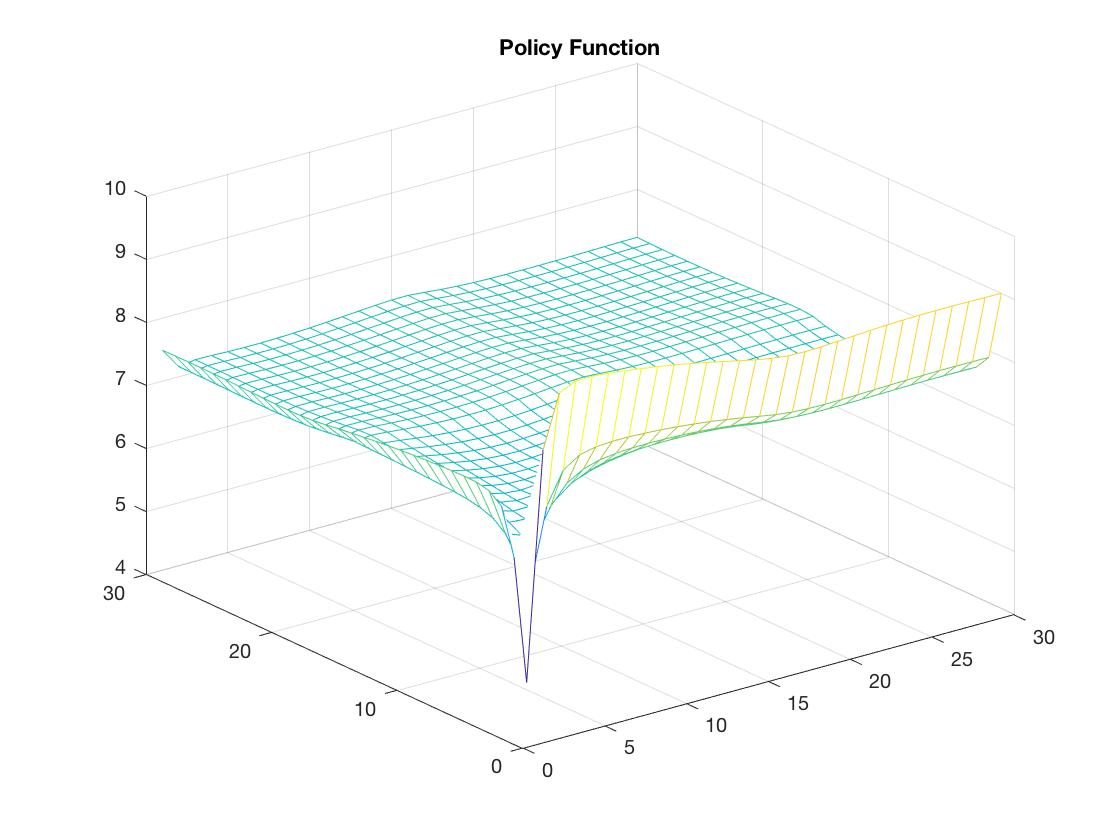
\includegraphics[scale=0.2]{Pol.jpg}

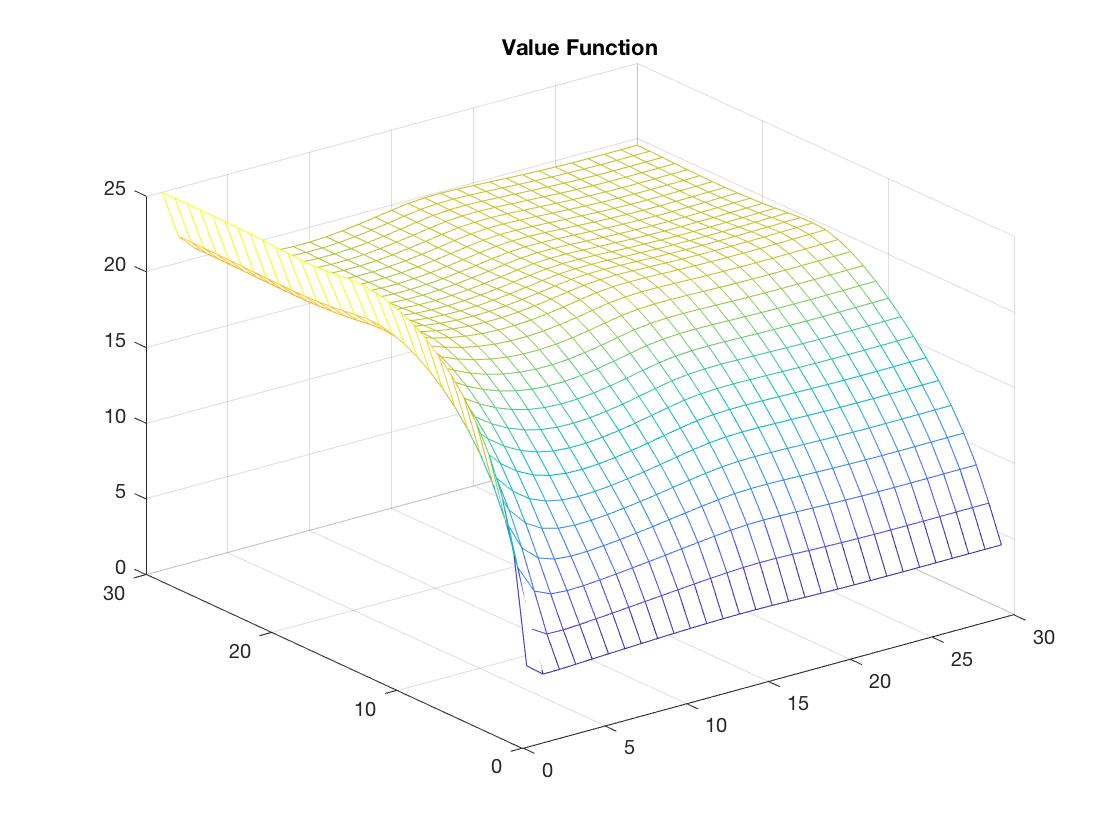
\includegraphics[scale=0.2]{val.jpg}


\item Starting from state (1,1), plot the distribution of states (a three dimensional plot) after 10, 20, and 30 periods.  
\item Compute and plot the the stationary distribution of states.
\end{enumerate}

%\newpage
%\bibliographystyle{dcu}
%\bibliography{$HOME/Dropbox/Papers/FullLib}

\end{document}
